\section{Introduction}

Spectrum Sensing is a key technology for Cognitive Radio. The initial task of any cognitive device, before any kind of dynamic spectrum management will be to accurately sense and classify spectral bands for availability. Dynamic management holds the promise of satisfying the almost ubiquitous growing demand for mobile and wireless data, with consumers demanding faster speeds and better quality connections in more places. However, there is constrained amount of frequencies over which to transmit this information; and demand for frequencies that provide sufficient bandwidth, good range and in-building penetration is high. Not all spectrum is used in all places and at all times, and judicious spectrum management, by developing approaches to use white spaces where they occur, would likely be beneficial.

Devices seeking to access white spaces need a robust mechanism for learning of the frequencies that can be used at a particular time and location. One approach is to refer to a database, which maps the location of white spaces based on knowledge of existing spectrum users. An alternative approach is for devices to detect white spaces by monitoring spectrum use. 

The advantages of spectrum monitoring \cite{akan2009cognitive} over persisting a database of space-frequency data are the ability of networks to make use of low-cost low-power devices, only capable of making local (as opposed to national) communications, keeping the cost of the network low and  opportunistic channel usage for bursty traffic, reducing channel collisions in dense networks. The main technical difficulty preventing spectrum sensing currently, are the high sampling rates required by wideband spectra such as TV white spaces (TVWS). However such spectra are typically sparse, in that transmissions use far fewer frequencies that the available bandwidth. 

Compressive Sensing (CS) \cite{Candes2006} has recently emerged as a new sampling paradigm, for acquiring sparse signals. Applying this to wireless communication, we are able to reconstruct sparse signals at sampling rates below what would be required by Nyquist theory, for example the works \cite{mishali2010theory}, \cite{polo2009compressive}, and \cite{tropp2010beyond} detail how this sampling can be achieved. 

However, even with CS, spectrum sensing from a single machine will be costly as the proposed TVWS band will be over a large frequency range CS at a single sensor would still require high sampling rates \cite{Zhang2011b}. In this paper we propose a distributed model, which allows a sensing budget at each node far below what is required by centralised CS. The advantages of such a network are that is should be able to average out noise process across some geographic area by making distributed observations, and make use of cheaper sensors due to the lowered sensing budget required per node. 

We cannot always guarantee that the frequency spectrum will always be sparse: for example, should TVWS become widely utilised, the spectra will not be sparse. However, even for highly occupied spectra, the gradient of the spectrum will be sparse. This has previously been exploited by \cite{tian2006wavelet}. 

Reconstructing the spectrum from compressive measurements could take place at a fusion centre, but such communications are expensive. It is more efficient therefore to design distributed algorithms where CRs communicate with their neighbours to reach consensus on the reconstruction, given each nodes' private data. However, regularising the reconstruction process would require global co-ordination if Total Variation (the \(l_1\) norm of the gradient of the signal) regularisation was chosen, as.

In this paper we propose a different model for sensing the gradient of the frequency spectrum to \cite{tian2006wavelet} - a model which doesn't require Total Variation regularisation of the objective function. 

We also propose a decentralised algorithm to solve the LASSO by consensus optimisation. This allows us to design an algorithm which requires no global co-ordination whilst reconstructing the gradient of the spectrum. We choose a convex approach, as convex algorithms require no knowledge of the signal statistics (such as sparsity), and are guaranteed to converge. We are able to find exact, closed form, expressions for the Distributed Lasso, reducing the computational load per iteration whilst obviating the need to approximate the objective function \cite{ling2015dlm}, \cite{mokhtari2015dqm}.

The structure of the paper is as follows: in section \ref{sec:sensingmodel} we introduce the sensing model, in section \ref{sec:opt-on-graphs} we describe the distributed reconstruction algorithm \cite{mota2013d}, and finally in section \ref{sec:results} we show some results of the reconstruction quality of this model. 

\section{Signal Model}

Not all signals are sparse in an orthogonal basis: for example, many images are sparse in an over-complete dictionary (set of bases). In particular, frequency spectra for TVWS may no longer be sparse once opportunistic radios begin operating in these frequency bands. 

Instead we aim to reconstruct the gradient of the spectrum, as we assume that transitions are constant within a band. Consider the basis defined by the function:

\begin{equation}
l_i\left(x\right) =
\begin{cases}
1 & \text{if } x \leq i \\
0 & \text{ otherwise } 
\end{cases}
\label{basis}
\end{equation}

That is, \(l_i\) is a left-hand step function. 

The basis (\ref{basis}) can be expressed as a matrix in \(\re^{n \times n}\) as:

\begin{equation}
L = \begin{pmatrix}
 1 & 0 & 0 & 0  & 0 \ldots 0 \\
  1 & 1 & 0 & 0  & 0 \ldots 0\\
     1 & 1 & 1 & 0  & 0 \ldots0  \\
    \ldots  \\
     1 & 1 & 1 & 1  & 1 \ldots 1 
\end{pmatrix}
\end{equation}

By direct computation, this inverse of \(L\) is:

\begin{equation}
D = \begin{pmatrix}
 1 & 0 & 0 & 0  & 0 \ldots 0 \\
  -1 & 1 & 0 & 0  & 0 \ldots 0\\
     0 & -1 & 0 & 0  & 0 \ldots0  \\
    \ldots  \\
     0 & 0 & 0 & 0  \ldots -1 & 1
\end{pmatrix}
\end{equation}

We model our PSD signal \(g\) as a linear combination of the basis functions (\ref{basis}):

\begin{equation}
g\left(x\right) = \sum_i a_i l_i\left(x\right) = L^Ta
\label{basis-expansion}
\end{equation}

where \(a = (a_1, \ldots, a_n\) are the coefficients in this basis expansion, and \(l_i\) are the rows of \(L\). Note that as defined, \(g\) is a column vector.

\begin{proposition}
\begin{equation}
D^Tg = a
\end{equation}
\label{def:a}
\end{proposition}
\begin{proof}

\begin{align}
D^Tg &= D^T L^T a \\
&= \left(LD\right)^Ta \\
&= a
\end{align}

as \(LD = I\).

\end{proof}

\section{Sensing Model}\label{sec:sensingmodel}

We consider a radio environment with a single primary user (PU) and a network of \(J\) nodes collaboratively trying to sense and reconstruct the PU signal in a fully distributed manner by local communication and regularisation only.

We try to sense and reconstruct a wideband signal, using a network of \(J\) (= 50) nodes placed uniformly at random within the square \(  \left[0,1\right]\times \left[0,1\right] \). 

We consider the frequency domain measurements, formed by each node mixing the signal with a random Gaussian signal \(A_j \in \re^n\). The measurements taken at node \(j\) are:

\begin{equation}
y_j = A_jH_jg + w_j
\label{dist_system}
\end{equation}

where \(H_j \in \re\) is the scalar channel gain, and \(w_j \sim \mathcal{N}(0,\sigma^2_n) \in \re \) is additive white Gaussian noise. 

For the purposes of comparison in section (\ref{sec:results}), this corresponds to the concatenated system:

\begin{equation}
y = AHg + w
\label{system}
\end{equation}

where \(H \in \re^{n \times n}\) is a block diagonal matrix of channel gains.

The system  \ref{system} can then be solved (in the sense of finding the sparse vector \(a\) (\ref{basis}) by convex optimisation via minimising the objective function:

\begin{equation}
\hat{a} = \argmin_{a} \frac{1}{2}\|AHL^{T}a-y\|_2^2 + \lambda \|a\|_1
\label{opt}
\end{equation}

where \(\lambda\) is a parameter chosen to promote sparsity. Larger \(\lambda\) means sparser \(a\).

\section{Constrained Optimisation on Graphs}\label{sec:opt-on-graphs}

We model the network of sensors as an undirected graph \(G = \left(V,E\right)\), where \(V = \{1 \ldots J\}\) is the set of vertices, and \(E = V \times V\) is the set of edges. An edge between nodes \(i\) and \(j\) implies that the two sensors can communicate. The set of nodes that node \(i\) can communicate with is written \(\mathcal{N}_i\) and the degree of node \(i\) is \(D_i = |\mathcal{N}_i|\). 

We assume that a proper colouring of the graph is available: that is, each node is assigned a number from a set \(C = \{1 \ldots c \} \), and no node shares a colour with any neighbour. This is so that nodes may communicate in colour order, as opposed to communicating individually thus reducing the total number of communication rounds required. 

Individually nodes make the following measurements (as discussed in section \ref{sec:sensingmodel}):

\begin{equation}
\vec{y}_j = \vec{M}_j\vec{x} + \vec{n}_j
\end{equation}

where \(\vec{M}_j = \left(\vec{AHL^T}\right)_j \) is the \(p^{th} \) row of the sensing matrix from \eqref{system}.

To find the \(\vec{x}\) we are seeking (the solution to \eqref{opt}, to each node we give a copy of \(\vec{x}\), \(\vec{x}_j \in \re^n\), and we constrain the copies to be identical across all edges in the network. To separate the minimisation of the \(\ell_2\) and \(\ell_1\) norms, we also introduce a dummy variable \(\vec{z}_j \in \re^n\) to each node. Each node, thus has a separate optimisation to solve, subject to the constraint that it is consistent with its neighbours.

We write the global optimisation variable as \(\bar{x}\), which collects together \(C\) copies of a \(n\times 1\) vector \(\vec{x}\):

\begin{defn}
We define vectors \(x_c\) which represent the subset of nodes with colour \(c\), where \(c = 1,\ldots , C\), and write the vector of length \(nJ\):
\begin{equation}
\bar{x} = \sum_{c=1}^C w_c \otimes x_c = \left[x_{c(1)}^T, \ldots	, x_{c(J)}^T\right]^T
\label{barxc}
\end{equation}
where \(w_{c(i)} = \mathbb{I}(c(i) = c)\), \(\mathbb{I}\) is the indicator function, and we have written \(c(i)\) for the colour of the \(i\)th node.
\end{defn}

The problem then is to solve:

\begin{align}
\argmin_{\bar{x}} \sum_{c=1}^C \sum_{j \in c} \|M_jx_j - y_j\|_2^2 + \frac{\lambda}{J}\|z\|_1 \nonumber \\ 
\text{ and } x_i = x_j \text{ if } \{i,j\} \in E \nonumber \\
\text{ and } x_i - z_i = \text{ } \forall i \in \{1, \ldots, C\}
\label{constrainedbp}
\end{align}

That is, at each node we minimise a Lasso functional constrained to be consistent across edges, but that is separable in the \(\ell_2\) and \(\ell_1\) norms.

The first set of constraints (edge-agreement) can be written more compactly by introducing the node-arc incidence matrix B: a \(V\) by \(E\) matrix where each column is associated with an edge \(\left(i,j\right) \in E\) and has \(1\) and \(-1\) in the \(ith\) and \(jth\) entry respectively. We require that \( Bx_j = 0 \) for all nodes \(j = 1, \ldots,  J\). The global constraint is simply \( (B \otimes I_n)\bar{x} = 0\), and using definition \eqref{barxc} the constraint \(x_i = x_j \text{ if } \{i,j\} \in E \) can now be written:

\begin{equation}
\sum_{c=1}^C\left(B_c^T \otimes I_n\right)\bar{x}_c = 0
\label{compact-constraints}
\end{equation}

note that \(\left(B^T\otimes I_n \right) \in \re^{nE \times nJ}\).

 Together \eqref{barxc} and \eqref{compact-constraints}, suggests that the problem \eqref{constrainedbp} can be re-written as:

\begin{align}
\argmin_{\bar{x}} \sum_{c=1}^C \sum_{j \in C_c} \|M_jx_j - y_j\|_2^2 + \beta\|z_j\|_1
\nonumber \\
\text{ s.t. } \sum_{c=1}^C\left(B_c^T \otimes I_n\right)\bar{x}_c = 0 \nonumber \\
\text{ and } \bar{x}_c - \bar{z}_c = 0
\label{constrainedbp1}
\end{align}

where \(\beta = \frac{\lambda}{J}\).

The global Augmented Lagrangian \cite{Boyd2010a}
 for the problem \eqref{constrainedbp1} can be written down as:

\begin{align}
L_\rho = \sum_{c=1}^C  \biggl( \sum_{j \in c} & \|M_jx_j - y_j\|_2^2 + \beta\|z_j\|_1  + \nonumber \\ & + \theta^T\left(\bar{x}_j - \bar{z}_j\right)  +  \frac{\rho}{2}\vectornorm{\bar{x}_j-\bar{z}_j}_2^2 \biggr) + \nonumber \\  & + \eta^T\left(B_c^T \otimes I_n\right)\bar{x}_c + \frac{\rho}{2}\vectornorm{\sum_{c=1}^C\left(B_c^T \otimes I_n\right)\bar{x}_c}_2^2
\label{aug-lagrange}
\end{align}

This is, superficially, similar to the Augmented Lagrangian for the Lasso problem \cite{Boyd2010a}[Section 6.4]. That is, the terms indexed by \(j\) are a straightforward Lasso problem, constrained by edge-wise variables (indexed by \(c\)) forcing consistency across the network. However, the problem (as currently written) is not separable across the edges of the network as the final and penultimate term represent the constraint that the nodes agree on their estimates across edges. 

To make it possible that \ref{aug-lagrange} can be posed  as a constrained optimisation problem at each node, we introduce the following variable:

\begin{defn}[Edge-equality vector]
\begin{align*}
u &:= \left(B^T \otimes I_n\right)\bar{x} \\
& = \left(B^T \otimes I_n\right)\sum_{c=1}^C w_c \otimes x_c \\
& = \sum	_{c=1}^C B_c^T\otimes x_c
\end{align*}
where we have used the definition \eqref{barxc} in the second line, the property of Kronecker products \((A\otimes C)(B \otimes D) = (AB \otimes CD)\) between the second and third lines, and we write \(B_c = w_c^TB\).
\end{defn}

The terms \(\|\sum_{c=1}^C\left(B_c^T \otimes I_n\right)\bar{x}_c\|^2\) and \( \eta^T\left(B_c^T \otimes I_n\right)\bar{x}_c \) of \eqref{aug-lagrange}, can be decomposed across edges, using the following lemma:

\begin{lemma}[Edge Decomposition]
\begin{equation}
\vectornorm{\sum_{c=1}^C\left(B_c^T \otimes I_n\right)\bar{x}_c}^2 = \sum_{j \in C_c}\left( D_j\vectornorm{x_j}_2^2 - \sum_{k \in \mathcal{N}_j} x_j^Tx^k\right)
\end{equation}

and

\begin{equation}
\eta^T\sum_{c=1}^C\left(B_c^T \otimes I_n\right)\bar{x}_1 = \sum_{l\in C_c} \sum_{m\in \mathcal{N}_l}\mathrm{sign}\left(m-l\right)\eta_{ml}^T x_l
\end{equation}

where \(\eta\) is decomposed edge-wise: \(\eta = \left(\ldots, \eta_{ij},\ldots\right)\), such that \(\eta_{i,j} = \eta_{j,i}\), and is associated with the constraint \(x_i = x_j\).


\begin{proof}
For the first part, note that 
\begin{align*}
u^Tu &= \vectornorm{\sum_{c=1}^C\left(B_c^T \otimes I_n\right)\bar{x}_c}^2 
\\ &=\sum	_{c_1=1}^C \sum	_{c_2=1}^C  \left(B_{c_1} \otimes x_{c_1}^T\right) \left(B_{c_2}^T \otimes x_c\right) \\
&= \sum_{c_1, c_2} B_{c_1}B_{c_2}^T \otimes x_{c_1}^Tx_{c_2}
\end{align*}

\(BB^T\) is a \(J \times J\) matrix, with the degree of the nodes on the main diagonal and \(-1\) in position \(\left(i,j\right)\) if nodes \(i\) and \(j\) are neighbours (i.e \(BB^T\) is the graph Laplacian). Hence, since we can write \(B_{c_1}B_{c_2}^T = w_{c_1}^TBB^Tw_{c_2}\), the trace of \(B_{c_1}B_{c_1}^T\) is simply the sum of the degrees of nodes with colour 1. Similar reasoning applies to all other colours.

For \(c_1 \neq c_2\),  \(B_{c_1}B_{c_2}^T\) corresponds to an off diagonal block of the graph Laplacian, and so counts how many neighbours each node with colour 1 has.

For the second part note that \(\eta \in \re^{nE}\) and can be written:

\begin{equation}
\eta = \sum_{c=1}^C w_c \otimes \eta_c
\end{equation}
where \(\eta_c\) is the vector of Lagrange multipliers associated across edges from colour \(c\). Now

\begin{align*}
\eta^Tu = \sum_{c_1=1}^C\sum_{c_2=1}^C w^T_{c_1}Bw_{c_2} \otimes \eta_{c_1}^Tx_{c_2}
\end{align*}
where we have repeated the reasoning from the previous part: using the properties of Kronecker products, and the definition of \(B_c\). For \(c_1=c_2\), \(\eta^Tu\) is zero, as there are no edges between nodes of the same colour by definition. For \(c_1\neq c_2\), \(\eta^Tu\) counts the edges from \(c_1\) to \(c_2\), with the consideration that the edges from \(c_2\) to \(c_1\) are counted with opposite parity. I.e. for a node \(l\) with colour \(C\), \(w_{c_1}^TB_{c_2}\) counts the edges to the neighbours of node \(l\), and the edges from the neighbours of node \(l\) to node \(l\) with opposite parity - \(\mathrm \sum_{l\in C_c} \sum_{m \in N_l} \mathrm{sign}(m-l)\).
\end{proof}
\end{lemma}

\begin{figure}
\begin{algorithmic}[1]
\Procedure{DADMM}{$y_j,M_j,\varepsilon$}
\State $x^0 = 0$, $z^0 = 0$, $\theta^0 = 0$, $\eta^0 = 0$, \\  $Q =  \left(M_j^TM_j + (\rho D_J + 1) I\right)^{-1}$, $w_j = M_j^Ty_j $
\While{$\vectornorm{z^{k+1} - z^{k}} \leq \varepsilon$}
\For{$c = 1, \ldots, C$}
\State $x^{k+1} \gets Q\left(w_j+  z^k - \theta^{kT} -\nu^{kT}\right)$  
\State  $z^{k+1} \gets S_{\beta/\rho}\left(x_j^{k+1} \right) $  
\State $\theta^{k+1}\gets \theta_j^{k} + \rho \left(x^{k+1}-z^{k+1}\right)$  
\EndFor
\\Each node transmits $x^{k+1}$ in $\mathcal{N}_j$ and calculates
  \State $\nu_j^{k+1} \gets \nu_j^k + \rho\left(\sum_{m \in N_j} z_m^k - z_j^k\right)$
\EndWhile
\State \textbf{return} $z^{k+1}$
\EndProcedure
\end{algorithmic}
\caption{The algorithm at Node \(j\)}\label{DADMM}
\end{figure}

Adding together this with the lemma, lets us write \eqref{aug-lagrange} as:

\begin{align}
L_\rho = \sum_{c=1}^C \biggl( \sum_{j \in C_c} \|M_jx_j - y_j\|_2^2 + \beta\|z_j\|_1 + \nu^Tx_j \nonumber \\
 + \theta\left(x_j - z_j\right) + \frac{\rho}{2}D_i\vectornorm{x_j}^2 + \frac{\rho }{2}\vectornorm{x_j-z_j}^2 \biggr)
\label{generic-iterations}
\end{align}

where we have defined:

\begin{equation}
\nu_i = \left(\sum_{k \in \mathcal{N}_i} sign\left(k-i\right)\eta_{\{i,k\}} - \rho x_k \right)
\end{equation}

which is a rescaled version of the Lagrange multiplier, \(\eta\), which respects the graph structure. 

Then by differentiating \eqref{generic-iterations} with respect to \(x_j\) and \(z_j\) we  can find closed forms for the updates as:

\begin{align}
x_j^{k+1} &:= \left(M_j^TM_j + (\rho D_J + 1) I\right)^{-1}\left(M_j^Ty_j +  z^k -\theta^{kT} - \nu^{kT}\right)\\
z_j^{k+1} &:= S_{\beta/\rho}\left(x_j^{k+1} \right)
 \\
\theta_j^{k+1} &:= \theta_j^{k} + \rho \left(x^{k+1}-z^{k+1}\right) \\
\nu_j^{k+1} &:= \nu_j^k + \rho\left(\sum_{m \in \mathcal{N}_j} z_m^k - z_j^k\right)
\label{dadmm_algo_lasso}
\end{align}

Where we have defined

\begin{defn}[Soft-thresholding]
\begin{equation}
S_{\tau}\left( y \right) := \mathrm{sign}(y)\mathrm{max}(y-|\tau|, 0)
\end{equation}
\end{defn}

\begin{remark}
This algorithm can be thought of as a distributed EM algorithm with memory: each node places a Gaussian prior with variance proportional to its degree on its private data, and solves a posterior least-squares problem. Each node then soft thresholds and then exchanges the result of this computation with its one-hop neighbours.
 
This explains the inclusion of an extra Lagrange multiplier: the multiplier \(\theta\) controls how far each node moves from its previous estimate in each iteration, whilst the multiplier \(\eta\) enforces consistency between nodes by integrating past disagreements between neighbouring nodes. Note that there is no communication of data between the nodes - only the result the computation in each round.
\end{remark}

\section{Results} \label{sec:results}

The model described in section \eqref{sec:sensingmodel}, equation \eqref{system} was simulated. The signal \(g \in \re^{300} \) was composed of 3 rectangular pulses, mimicking primary user signals in TVWS, as shown in figure \eqref{different_sigs} (a). The signal was put through a Rayleigh channel, before being sensed by the nodes. The network was generated as a random geometric graph in \([0,1] \times [0,1]\), with 50 nodes. If the network wasn't connected, it was redrawn. 200 mixing patters were drawn i.i.d from a \(\mathcal{N}\left(0, \sigma^2 I_{300} \right) \) distribution, with \(\sigma^2 = 1/200\), to from the matrix \(A\in  \re^{200 \times 300}\).

Monte Carlo simulations were performed at 18 \(\sigma^2_n\) values ranging from 1 to 10 and the expected Mean Squared Error (MSE) of solutions of a centralised ADMM solver and a our distributed solver were calculated over 500 repetitions with 1200 iterations (\(k\)) per repetition.

The MSE was calculated as follows:

\begin{equation}
\frac{\vectornorm{L^tz^k - g^*}}{\vectornorm{g^*}}
\end{equation}

where \(z^k\) is the result of the algorithm at iteration \(k\), and \(g^*\) is the optimal solution.

The SNR for each repetition was calculated as

\begin{equation}
\frac{\vectornorm{g^*}}{\vectornorm{w}}
\end{equation}

and averaged over the 500 repetitions. The results are shown in figure \eqref{msevssnr0}. Following \cite{Chen1998}, for each repetition we chose 

\begin{equation}
\lambda = \sqrt{2\sigma^2_n\log{n}}
\end{equation}

The error bars indicate the empirical variance across the 500 repetitions.

These results indicate that for both the centralised and distributed solvers, their performance degrades as the noise power increases in a roughly log-linear fashion. The performance of the distributed algorithm is consistently worse than the centralised version, this contrasts with results from \cite{bazerque2008}; this is due to the differing sparsity models: \cite{bazerque2008} use a joint space and frequency model for the sparsity, and as such observe an spatial averaging out of noise when using a distributed solver. The performance of DADMM is within the error bars of the centralised version at low SNR, and gap in performance between the two versions is no more than \(10^{-2}\). Even at relatively lower SNRs both solvers reach a solution within \(10^{-1}\) of the optimal (as measured by normalised MSE), which will be adequate for the task of spectrum sensing. For example the reconstructions in figures \eqref{different_sigs} (c) and (d) show realisations of the reconstruction from DADMM with \(\sigma^2_n = 5\) and \(\sigma^2_n = 20\) respectively. It is still possible to distinguish the occupied bands from unoccupied frequencies for both reconstructions.

The distributed algorithm has consistently larger variance, than the centralised solver at all SNRs. This is due to individual nodes only having access to a subset of the data to perform calculations on: the variance will be proportional to the square-root of number of data samples at each node, which are fewer than the total number of samples available to the centralised solver. 

In figure \eqref{fig:differentLambda}, we plot the progress of DADMM along the solution path for a variety of regularisation parameters \(\lambda\). The y-axis is the relative (unormalised) MSE between the optimal solution and the current iteration, and the x-axis is the iteration number. We note that for a fixed \(\lambda\) there is a single unique optimal solution, which DADMM converges to (in the sense of stationary error between consecutive iterations). This solution may not be attained in the allotted number of iterations, as the rate of convergence is determined by \(\lambda\), \(\rho\) and the eigenvalues of the Laplacian of \(G\). The paper \cite{shi2014linear}, proves linear convergence for DADMM, with explicit expressions for the rate. In particular the rate convergence of DADMM is affected by the choice of \(\lambda\): smaller \(\lambda\) corresponds to slower convergence - this is intuitive as solutions with fewer non-zero components should require fewer iterations to fully specify. Notice that for some \(\lambda\)s the solution path exhibits phenomenological  behaviour similar to damped oscillations: this phenomena has been explored in \cite{nishihara2015general} and \cite{su2014differential}.  

\begin{figure}[h]
\centering
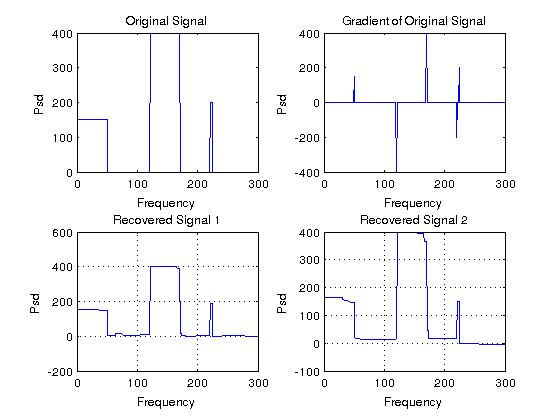
\includegraphics[height = 7.3 cm]{signal_and_recovery.jpg}
\caption{Left to right: (a) The original signal. (b) The gradient \eqref{def:a} of the original signal. (c) Recovery using DADMM, 1000 iterations, \(\sigma^2_n = 5\). (d) Recovery using DADMM, 1000 iterations, \(\sigma^2_n = 20\)  }
\label{different_sigs}
\end{figure}

\begin{figure}[h]
\centering
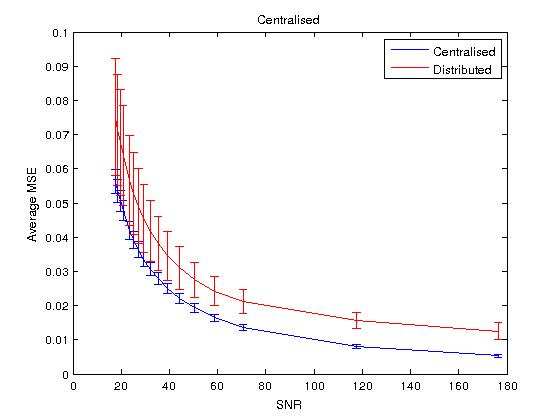
\includegraphics[height = 7.3 cm]{Cent_Vs_Distrib_snr.jpg}
\caption{MSE vs SNR for the sensing model showing the performance of distributed and centralised solvers. The performance of DADMM is consistently within \(10^{-2}\) of ADMM, and within the error bars of ADMM at low SNRs. The variance of estimates produced by DADMM is larger than ADMM, due to nodes performing computations on a subset of data. Both estimates are consistently within \(10^{-1}\) of the optimal solution, which is sufficient to classify occupied bands.} 
\label{msevssnr0}
\end{figure}

\begin{figure}[h]
\centering
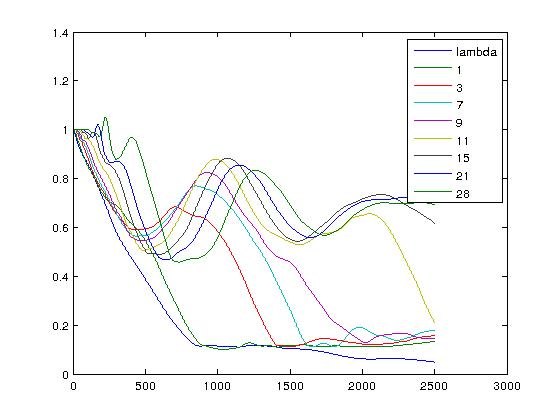
\includegraphics[height = 7.3 cm]{continuations_errors.jpg}
\caption{The progress of the distributed solver as a function of the number of iterations, with different values of the regression parameter \( \lambda \). For a fixed \( \lambda \) there is a single unique optimal solution, with higher \( \lambda \) favouring sparser solutions. The convergence of DADMM is slowed by smaller \( \lambda \). This is intuitive: solutions with fewer non-zero components should be identified in fewer iterations.}
\label{fig:differentLambda}
\end{figure}

\section{Conclusions}
We have demonstrated an alternating direction algorithm for distributed optimisation with exact (as opposed to linear or quadratic approximations to the objective as in \cite{mokhtari2015dqm} and \cite{ling2015dlm}) closed form expressions for the computation at each iteration, and discussed the statistical properties of the estimation. 

We have simulated the performance of this distributed algorithm for the distributed estimation of frequency spectra, in the presence of additive (white, Gaussian) and multiplicative noise. We have shown that the algorithm is robust to a variety of SNRs and converges to a similar solution as an equivalent centralised algorithm (in relative mean-squared-error).

We plan to work on larger, more detailed, models for the frequency spectra, to extend our regression framework to solve the MMV problem, to accelerate the convergence via Nesterov type methods to smooth the convergence of the distributed algorithm \cite{goldstein2014fast}, and to incorporate spatial variation into our model to further promote sparsity. We also plan to automate the choice of \(\lambda\) via continuation methods, and study how the choice of \(\lambda\) and \(\rho\) affect the rate of convergence. 